% =============================================================
% Capítulo 4 - Diseño del circuito de detección de picos
% =============================================================
\chapter{Diseño del circuito de detección de picos}
\label{cap:diseno_deteccion_picos}

Para determinar el valor máximo de la señal de salida del fotodiodo correspondiente al lazo de sintonización se plantearon dos alternativas tecnológicas:

\begin{itemize}
  \item Digitalizar la señal completa mediante un conversor analógico-digital (ADC) de alta velocidad y procesarla posteriormente por software para localizar el valor máximo.
  \item Retener el valor máximo de la señal analógica mediante un circuito detector de picos y digitalizar dicho valor con un ADC de menor velocidad.
\end{itemize}

Por razones de costo e implementación, se adoptó la segunda alternativa, ya que permite emplear un ADC de menor velocidad de muestreo y costo reducido, disminuyendo simultáneamente el volumen de datos a procesar por el microcontrolador.

\section{Modelado del circuito de detección}
\label{sec:modelado_simulacion}

El circuito detector de picos diseñado consta de dos amplificadores realimentados por corriente (CFA), conectados en configuración no inversora, y un transistor bipolar que opera como elemento detector y buffer de carga. 

En la Figura \ref{fig:detector} se ilustra el esquema eléctrico del detector propuesto para el canal $P_+$. El amplificador $\text{U1A}$ está configurado como no inversor con una ganancia $G = +2$, donde la resistencia $R_1$ adapta la impedancia proveniente del amplificador de transimpedancia del fotodetector. El transistor $Q_1$ se emplea como diodo detector mediante su unión base-emisor y se encarga de cargar el circuito $RC$ conformado por $R_3$ y $C_1$. El amplificador $\text{U1B}$ actúa como separador (\emph{buffer}) de salida con ganancia unitaria, evitando que la impedancia de entrada del ADC descargue el capacitor de retención antes de completar la conversión. El empleo de integrados CFA, en lugar de los amplificadores realimentados por tensión (VFA) convencionales, permite alcanzar un elevado \emph{slew rate}, condición determinante para seguir la rápida variación temporal de la señal proveniente del fotodiodo.

\begin{figure}[h]
  \centering
  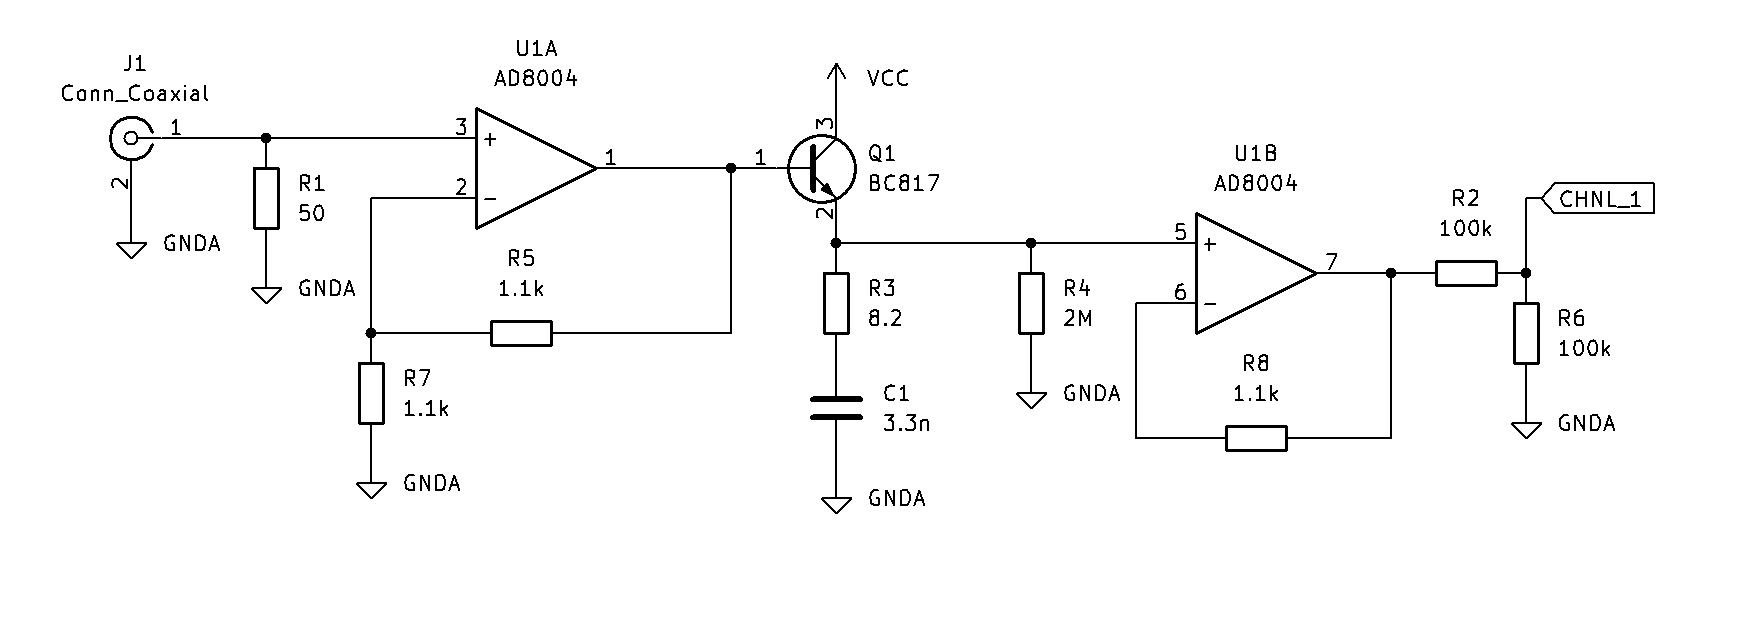
\includegraphics[width=0.8\textwidth]{figuras/4_detectordepicos.png}
  \caption{Circuito detector de picos para el canal $P_+$ (Fuente: elaboración propia).}
  \label{fig:detector}
\end{figure}

El amplificador $\text{U1A}$ se configuró con una ganancia de 2 para extender el rango dinámico del circuito. Ante niveles bajos de señal a la entrada del detector (derivados de una atenuación severa del haz láser), se presentan dos limitaciones principales: la no linealidad intrínseca de la unión base-emisor del transistor a bajas corrientes y la excursión máxima de salida (\emph{Output Voltage Swing}) del amplificador operacional. De esta forma, se logra un compromiso adecuado entre la linealidad del circuito para niveles altos de excitación y la sensibilidad a señales débiles.

Partiendo de la ecuación diferencial de carga de un circuito $RC$,

\begin{equation}
  V_C(t) = V_O \left(1 - e^{-\frac{t}{R_3 C_1}}\right)
  \label{eq:carga_rc}
\end{equation}

\noindent y considerando que para tiempos $t / (R_3 C_1) \ll 1$ la exponencial puede aproximarse mediante su serie de Taylor de primer orden como:

\begin{equation}
  V_C(t) \approx V_O \, \frac{t}{R_3 C_1},
  \label{eq:carga_rc_lineal}
\end{equation}

\noindent se obtiene una relación lineal entre la tensión retenida y la tensión de pico de entrada sin necesidad de cargar completamente el capacitor $C_1$. Esto permite seleccionar valores de capacidad que otorguen tiempos de descarga suficientemente prolongados para digitalizar el valor de pico $V_O$ empleando un conversor de velocidad moderada.

\section{Selección de componentes activos}

El amplificador realimentado por corriente AD8004 fue seleccionado debido a su elevado \emph{slew rate} (resumido en la Tabla \ref{tab:caracteristicas_ad8004}) y su bajo costo. La integración de cuatro amplificadores operacionales en un mismo encapsulado permite reducir la superficie de la placa y garantizaría, por lo menos en teoría, que ambos canales experimenten la misma deriva térmica.

\begin{table}[h]
  \centering
  \begin{tabular}{lll}
    \toprule
    \textbf{Parámetro} & \textbf{Valor} & \textbf{Condiciones} \\
    \midrule
    \multicolumn{3}{l}{\textit{Desempeño dinámico}} \\
    Ancho de banda ($-3$~dB)            & 250~MHz             & $G = +1$          \\
    Ancho de banda (planitud 0,1~dB)    & 30~MHz              & $G = +2$          \\
    Slew rate                           & 3000~V/\textmu s   & $V_S = \pm5$~V    \\
    Slew rate                           & 1100~V/\textmu s   & $V_S = +5$~V      \\
    Tiempo de establecimiento (0,1\,\%) & 21~ns               &                   \\
    Tiempo de subida (escalón de 2~V)   & 1,8~ns              &                   \\
    \midrule
    \multicolumn{3}{l}{\textit{Desempeño DC y características de entrada}} \\
    Tensión de \emph{offset} de entrada     & 1,0~mV (típ.); 3,5~mV (máx.) &                \\
    Corriente de polarización de entrada    & $\pm40$~\textmu A (típ.)      &                \\
    Transresistencia en lazo abierto        & 290~k$\Omega$                & $V_O = \pm2.5$~V \\
    Resistencia de entrada (no inversora)   & 2~M$\Omega$                  &                \\
    Rango de tensión de entrada (modo común)& 3,2~V                        &                \\
    \midrule
    \multicolumn{3}{l}{\textit{Salida y alimentación}} \\
    Corriente de salida                     & 50~mA               &                        \\
    Corriente de alimentación por amplif.   & 3,5~mA (35~mW)      &                        \\
    Rango de alimentación (simple)          & +4 a +12~V          &                        \\
    Rango de alimentación (dual)            & $\pm2$ a $\pm6$~V   &                        \\
    Tensión de alimentación máxima          & 12,6~V              & Valor máximo absoluto  \\
    Rango de temperatura de operación       & $-40$ a $+85$~$^{\circ}$C & Grado A          \\
    Encapsulado                             & SOIC de 14 pines    &                        \\
    \bottomrule
  \end{tabular}
  \caption{Características principales del amplificador realimentado por corriente AD8004 (Fuente: adaptado de \cite{ad8004_ds}).}
  \label{tab:caracteristicas_ad8004}
\end{table}

Como elemento detector se empleó un transistor bipolar NPN BC817, cuya alta capacidad de corriente de colector ($I_C = 500\,\text{mA}$, véase la Tabla \ref{tab:caracteristicas_bc817}) resulta indispensable para cargar rápidamente el capacitor acoplado a su emisor.

\begin{table}[h]
  \centering
  \begin{tabular}{lll}
    \toprule
    \textbf{Parámetro} & \textbf{Valor} & \textbf{Condiciones} \\
    \midrule
    \multicolumn{3}{l}{\textit{Valores máximos absolutos}} \\
    Tensión colector-base ($V_{CBO}$)   & 50~V             & $I_E = 0$        \\
    Tensión colector-emisor ($V_{CEO}$) & 45~V             & $I_B = 0$        \\
    Tensión emisor-base ($V_{EBO}$)     & 5~V              & $I_C = 0$        \\
    Corriente de colector ($I_C$)       & 500~mA           & Continua         \\
    Potencia de disipación ($P_D$)      & 300~mW           & $T_A = 25$~$^{\circ}$C \\
    Temperatura de unión ($T_J$)        & 150~$^{\circ}$C  & Máxima           \\
    \midrule
    \multicolumn{3}{l}{\textit{Características eléctricas}} \\
    Ganancia de corriente DC ($h_{FE}$)      & 160 a 400            & $V_{CE}=1$~V, $I_C=100$~mA \\
    Tensión de saturación C-E ($V_{CE(\text{sat})}$)& 0,7~V (máx.)         & $I_C=500$~mA, $I_B=50$~mA  \\
    Tensión de saturación B-E ($V_{BE(\text{sat})}$)& 1,2~V (máx.)         & $I_C=500$~mA, $I_B=50$~mA  \\
    Frecuencia de transición ($f_T$)         & 100~MHz (mín.)       & $V_{CE}=5$~V, $I_C=10$~mA  \\
    \midrule
    \multicolumn{3}{l}{\textit{Datos generales}} \\
    Tipo        & NPN de silicio, propósito general & \\
    Encapsulado & SOT-23                            & \\
    \bottomrule
  \end{tabular}
  \caption{Características principales del transistor bipolar NPN BC817 (Fuente: adaptado de \cite{bc817_ds}).}
  \label{tab:caracteristicas_bc817}
\end{table}

\section{Selección de componentes pasivos}

Para el dimensionamiento de los componentes pasivos del circuito se consideraron los siguientes criterios de diseño:
\begin{itemize}
  \item La resistencia de polarización de emisor $R_4$ debe ser suficientemente alta para no descargar el capacitor $C_1$ antes de la conversión analógico-digital, pero adecuada para establecer un punto de operación estable en reposo.
  \item La constante de tiempo $\tau = R_3 C_1$ debe garantizar la aproximación lineal descrita en la Ecuación \ref{eq:carga_rc_lineal} durante el pulso de entrada. Este criterio es el que fija el valor de $R_3$.
  \item La corriente de pico que impone $R_3$ sobre el transistor $Q_1$ debe resultar admisible para el régimen impulsivo de trabajo, lo que se verifica en términos de energía por pulso y potencia media disipada.
  \item Las redes de realimentación para $\text{U1A}$ y $\text{U1B}$ se ajustaron según las recomendaciones del fabricante del AD8004 para optimizar la respuesta en frecuencia y asegurar la estabilidad en lazo cerrado.
\end{itemize}

\subsection{Cálculo de la constante de tiempo del circuito RC}

A partir de las caracterizaciones experimentales de la señal entregada por los fotodetectores se determinó que el pulso útil tiene una duración aproximada de $2\,\text{ns}$, seguido de un decaimiento exponencial que ya no contribuye a la carga del capacitor de retención. Para que dicha carga permanezca en la zona lineal descrita por la Ecuación \ref{eq:carga_rc_lineal} debe cumplirse $t \ll \tau = R_3 C_1$, condición que fija un valor objetivo de constante de tiempo del orden de las decenas de nanosegundos.

Adoptando un valor comercial E24 estándar de $R_3 = 8{,}2\,\Omega$ junto con un capacitor $C_1 = 3{,}3\,\text{nF}$, se obtiene una constante de tiempo efectiva de:

\begin{equation}
  \tau = R_3 C_1 = 8{,}2\,\Omega \times 3{,}3\,\text{nF} = 27{,}06\,\text{ns}
  \label{eq:tau_final}
\end{equation}

Fijado $R_3$ por el criterio anterior, queda verificar que la corriente que atraviesa el transistor $Q_1$ sea admisible. El valor adoptado impone una corriente de pico inicial:

\begin{equation}
  I_0 = \frac{V_{O,\text{U1A}} - V_{BE}}{R_3} = \frac{12\,\text{V} - 1{,}2\,\text{V}}{8{,}2\,\Omega} = 1{,}32\,\text{A}
  \label{eq:valor_r3_calc}
\end{equation}

\noindent valor superior a la corriente máxima de pico $I_{CM} = 1\,\text{A}$ que declara la hoja de datos del BC817 \cite{bc817_ds}. Dicho límite, sin embargo, está especificado para pulsos de $20\,\text{ms}$, un régimen en el que el calor generado alcanza a difundir hacia el encapsulado y la restricción es de naturaleza térmica. En la aplicación presente el pulso dura $2\,\text{ns}$, seis órdenes de magnitud menos, por lo que corresponde verificar la disipación efectiva en lugar de aplicar el límite de forma directa.

Con una caída colector-emisor $V_{CE} \approx 1{,}2\,\text{V}$ y una corriente media de $1{,}27\,\text{A}$ durante el pulso, la potencia instantánea alcanza $1{,}58\,\text{W}$ y la energía depositada en la juntura por cada disparo resulta:

\begin{equation}
  E_{pulso} = V_{CE}\, \bar{I}_C\, t = 1{,}2\,\text{V} \times 1{,}27\,\text{A} \times 2\,\text{ns} = 3{,}05\,\text{nJ}
  \label{eq:energia_pulso_q1}
\end{equation}

A la frecuencia de repetición del láser de $20\,\text{Hz}$, el ciclo de trabajo es de $4\times10^{-8}$ y la potencia media disipada por $Q_1$ asciende a $61\,\text{nW}$, seis órdenes de magnitud por debajo de los $250\,\text{mW}$.

 El transistor opera por lo tanto muy lejos de su límite térmico, y el valor de $I_{CM}$ de la hoja de datos debe interpretarse como una cota de régimen continuo y no como una restricción activa del diseño.


\subsection{Cálculo de la red de polarización del transistor}

El transistor $Q_1$ opera en configuración seguidor de emisor (colector común), actuando como buffer de tensión que permite al amplificador $\text{U1A}$ cargar el nodo capacitivo con valores pico superiores a la capacidad de salida del propio OPAMP.

Dado que la etapa no cuenta con excursión \emph{rail-to-rail}, en ausencia de señal de entrada la tensión de salida continua en reposo del $\text{U1A}$ es de aproximadamente $1\,\text{V}$. Para evitar la descarga prematura del capacitor de retención a través de $R_4$, se impuso la condición $R_4 \gg R_3$, seleccionándose $R_4 = 82\,\text{k}\Omega$.

La corriente de reposo de emisor resulta:

\begin{equation}
  I_E = \frac{V_{O,\text{U1A}} - V_{BE}}{R_4} = \frac{1\,\text{V} - 0{,}58\,\text{V}}{82\,\text{k}\Omega} = 5{,}12\,\mu\text{A}
  \label{eq:transistor_ie}
\end{equation}

Cabe señalar que la tensión base-emisor empleada en la Ecuación \ref{eq:transistor_ie} difiere de la utilizada en la Ecuación \ref{eq:valor_r3_calc}. Ello responde a que $V_{BE}$ depende de la corriente de colector: el valor de $1{,}2\,\text{V}$ corresponde al régimen impulsivo de amperes durante el pico, mientras que los $0{,}58\,\text{V}$ corresponden al régimen de reposo, de algunos microamperes.

Esta pequeña corriente de polarización mantiene al transistor en el límite de la zona activa sin comprometer la retención de carga en $C_1$. En la Tabla \ref{tab:componentes_pasivos} se resumen los valores y características de los componentes pasivos adoptados.

\begin{table}[h]
  \centering
  \begin{tabular}{c c c c l}
    \toprule
    \textbf{Componente} & \textbf{Valor} & \textbf{Tolerancia} & \textbf{Encapsulado} & \textbf{Función técnica} \\
    \midrule
    $R_1$ & $50\,\Omega$ & $\pm 1\%$ & SMD 0603 & Adaptación de impedancia de entrada \\
    $R_2$ & $1\,\text{k}\Omega$ & $\pm 1\%$ & SMD 0603 & Red de realimentación U1A ($G=+2$) \\
    $R_3$ & $8{,}2\,\Omega$ & $\pm 1\%$ & SMD 0603 & Limitador de corriente de carga del capacitor \\
    $R_4$ & $82\,\text{k}\Omega$ & $\pm 1\%$ & SMD 0603 & Polarización de reposo de emisor ($Q_1$) \\
    $R_f$ & $1\,\text{k}\Omega$ & $\pm 1\%$ & SMD 0603 & Resistencia de lazo CFA (estabilidad U1A/U1B) \\
    $C_1$ & $3{,}3\,\text{nF}$ & $\pm 5\%$ & SMD 0603 (NP0/C0G) & Capacitor de retención de tensión de pico \\
    \bottomrule
  \end{tabular}
  \caption{Componentes pasivos seleccionados para el circuito detector de picos (Fuente: elaboración propia).}
  \label{tab:componentes_pasivos}
\end{table}

\section{Simulación del circuito detector de picos}
\label{sec:simulacion_circuito_detector}

La simulación del circuito se ejecutó tomando como señal de excitación una captura osciloscópica real de la salida del fotodiodo (Figura \ref{fig:pulso}). Como entorno de simulación se utilizó el motor NGSPICE v46 integrado con la interfaz gráfica QUCS-S (Figura \ref{fig:sim}).

\begin{figure}[htbp]
  \centering
  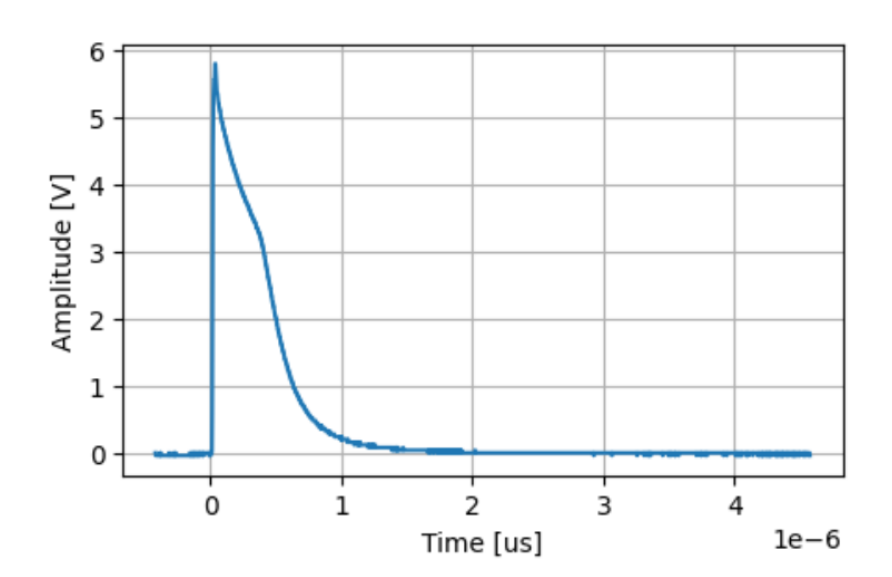
\includegraphics[width=0.6\textwidth]{figuras/4_señalpulso.png}
  \caption{Señal pulsada $P_+$ capturada mediante osciloscopio Tektronix (Fuente: elaboración propia).}
  \label{fig:pulso}
\end{figure}

\begin{figure}[htbp]
  \centering
  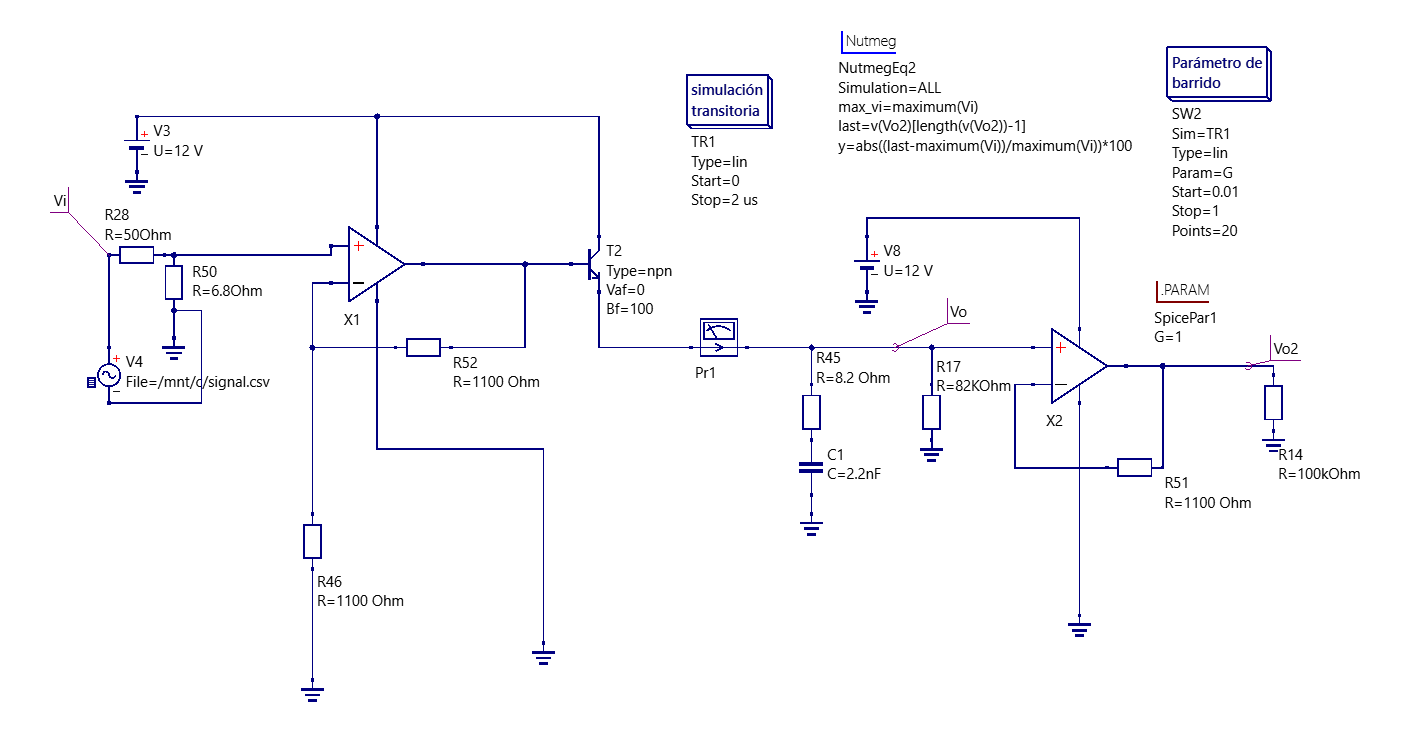
\includegraphics[width=1\textwidth]{figuras/4_simulacion.png}
  \caption{Esquema del circuito detector implementado en QUCS-S (Fuente: elaboración propia).}
  \label{fig:sim}
\end{figure}

Se ejecutó un análisis de barrido paramétrico (\emph{DC/Transient sweep}) de 25 valores de tensión de entrada $V_{\text{in}}$ (Figura \ref{fig:barrido}). Los resultados confirman una respuesta lineal para tensiones de entrada $V_{\text{in}} \ge 0{,}8\,\text{V}$ (Figura \ref{fig:linealidad}), límite impuesto por el piso de tensión del amplificador operando bajo fuente simple de $+12\,\text{V}$.

\begin{figure}[htbp]
  \centering
  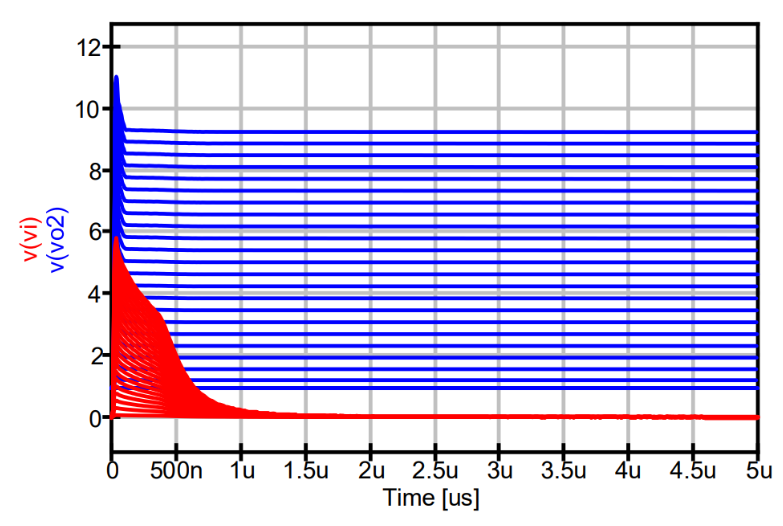
\includegraphics[width=0.7\textwidth]{figuras/4_simbarrido.png}
  \caption{Barridos temporales de la tensión de salida para distintos niveles de $V_{\text{in}}$ (Fuente: elaboración propia).}
  \label{fig:barrido}
\end{figure}

La tensión retenida por el detector fue evaluada a los $5\,\mu\text{s}$ posteriores al pico de entrada. Este intervalo responde al tiempo necesario para que un ADC comercial de costo moderado (con tasa de muestreo de $500\,\text{ksps}$) realice el ciclo de muestreo y retención (\emph{Sample \& Hold}) sin introducir errores temporales.

\begin{figure}[htbp]
  \centering
  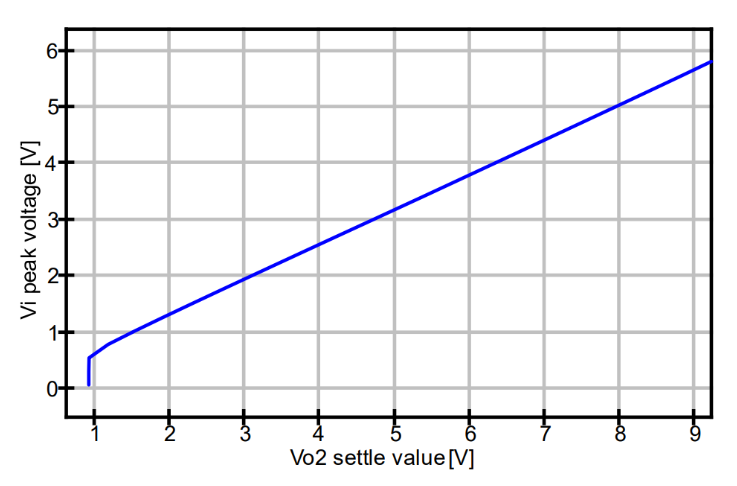
\includegraphics[width=0.7\textwidth]{figuras/4_simlinealidad.png}
  \caption{Tensión de salida $V_O$ medida a $t = 5\,\mu\text{s}$ en función de la tensión de pico de entrada $V_{\text{in}}$ (Fuente: elaboración propia).}
  \label{fig:linealidad}
\end{figure}

Este rango de operación se considera correcto como se verá en el Capítulo \ref{cap:modelo_experimental}, puesto que los valores de tensión que realmente importan para controlar el HSRL son definidos a criterio del operador, en torno a los mínimos de $P_+$ y $P_-$. Además, poseemos dos grados de libertad para mantenernos en la zona lineal del detector, relacionados con la intensidad de los haces de referencia:

\begin{itemize}
  \item Densidad óptica del filtro neutro, mostrado en la figura \ref{fig:diagrama_hsrl}.
  \item Absorción óptica de la celda de iodo de referencia, explicado en el Capítulo \ref{cap:lidar_hsrl}.
\end{itemize}

\section{Prototipado y validación experimental}
\label{sec:prototipado_validacion}

Se fabricó un primer prototipo en laboratorio mediante la técnica de transferencia térmica y grabado químico con cloruro férrico. Se montaron componentes de tecnología de montaje superficial (SMD) para minimizar el impacto de las componentes parásitas.

Al someter el circuito a un pulso de prueba de $100\,\text{ns}$ de ancho a una frecuencia de repetición de $20\,\text{Hz}$, la respuesta temporal presentó oscilaciones severas en el nodo de salida (véase la Figura \ref{fig:oscilaciones}). Este comportamiento inestable fue provocado por capacidades parásitas acopladas a los nodos de alta impedancia de los amplificadores CFA, degradando fuertemente la linealidad del detector.

\begin{figure}[htbp]
  \centering
  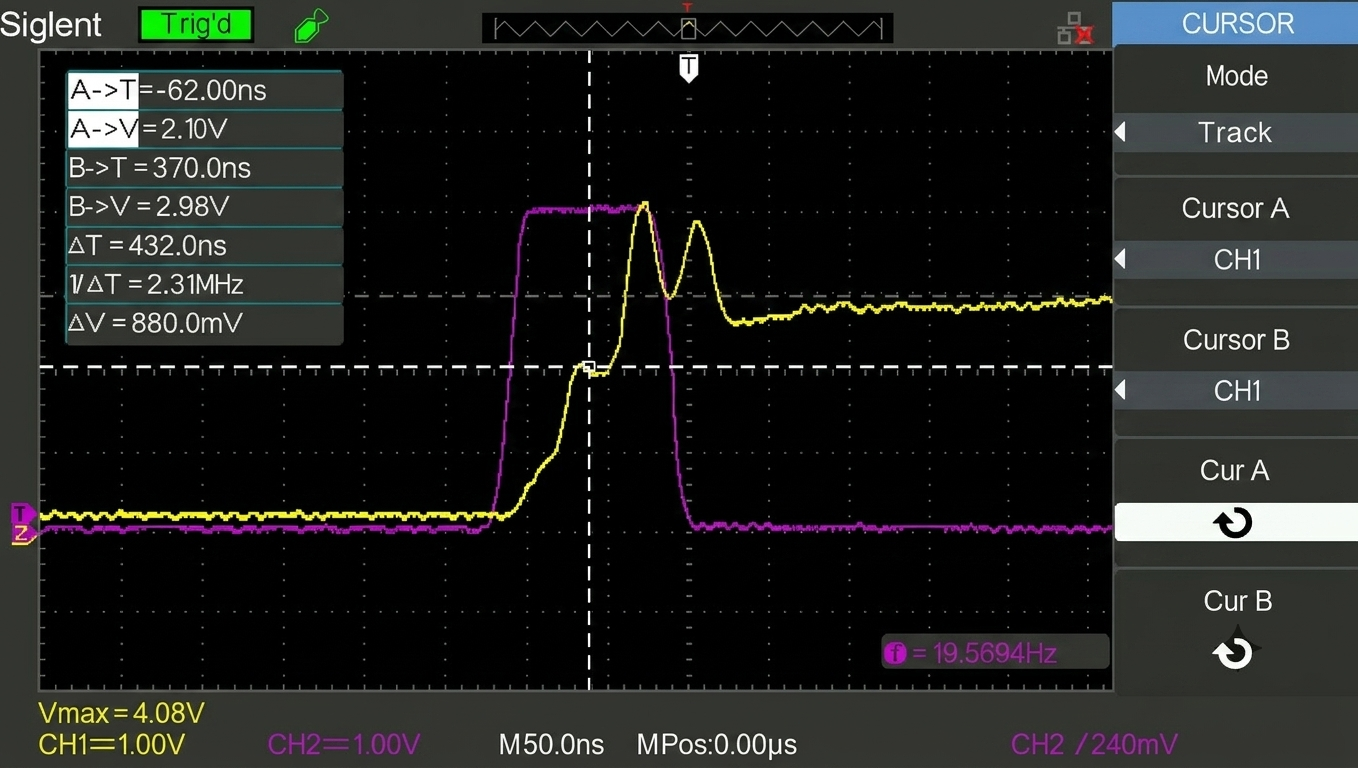
\includegraphics[width=0.8\textwidth]{figuras/4_oscilacion.png}
  \caption{Respuesta del prototipo ante un pulso de $100\,\text{ns}$ ($20\,\text{Hz}$), evidenciando oscilaciones de alta frecuencia derivadas de parásitos del trazado (Fuente: elaboración propia; imagen procesada con inteligencia artificial \cite{nanobananapro}).}
  \label{fig:oscilaciones}
\end{figure}

Ante esta problemática, previo a continuar con los ensayos en laboratorio, se decidió diseñar un nuevo circuito impreso (PCB) multicapa optimizado para aplicaciones de alta frecuencia. En esta fase integradora se incorporaron también el microcontrolador de control del sistema (desarrollado en la Sección \ref{sec:rp2350}) y los transceptores para la interfaz de comunicación serie con el sistema \emph{seeder} (Sección \ref{sec:rs232_uart}).

El análisis detallado sobre el diseño de la placa final y validación del circuito analógico se desarrolla en mayor detalle en el Capítulo \ref{cap:placacontrol}.

